\section{Theory}
	To begin, the droplets are free to fall in the gravitational field. Because the droplet is also being forced upon by the viscous force caused by air particles, it will balance its weight if the droplet is tiny enough. The masses and radii of the droplets may be calculated by solving for the forces. The potential difference is now activated, and the negatively charged droplets begin to move upwards towards the positively charged top plate, while the positively charged droplets accelerate downwards. If the size and charge of the droplets allow, the negative droplet should reach its terminal velocity as the electric and viscous forces balance the droplet's weight. The charge on the droplet may now be calculated using the early discovered radii values. To reduce random errors, measurements are repeated using the same droplet. A droplet of small size and low charge should be found for the experiment.

	\begin{figure}[H]
		\centering
		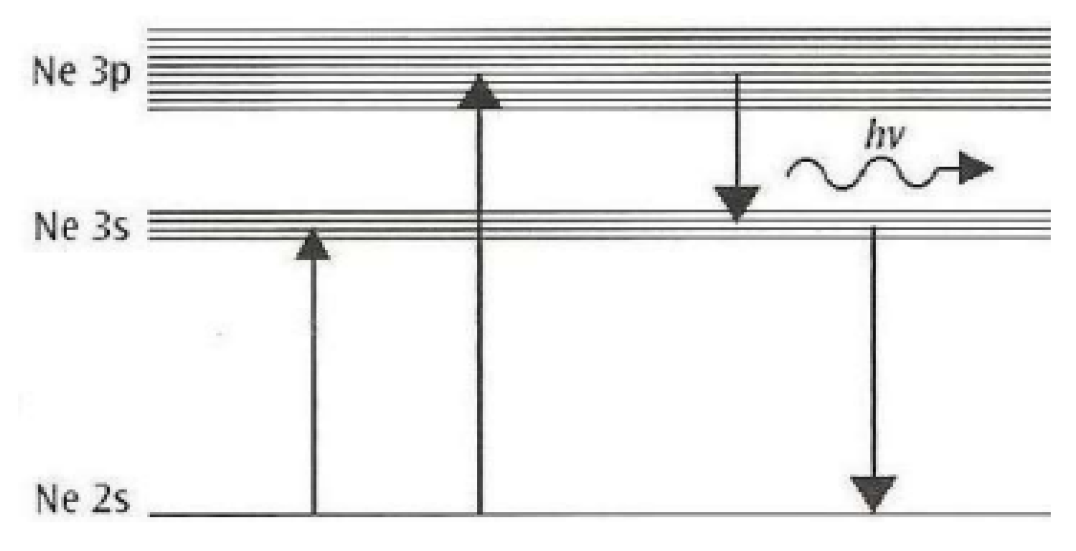
\includegraphics[width=0.3\textwidth]{1.png}
		\caption{\textbf{(a) Dynamic Method, (b) Balancing Method}}
		\label{fig:1}
	\end{figure}

	Consider a droplet of radius r travelling with a terminal fall velocity of v in the absence of potential. The density of oil is $\rho$, while the density of air is $\rho_a$. As a result, the forces can be balanced as follows:

	$$\frac{4\pi(\rho-\rho_a)r^3g}{3} = 6\pi r\eta v_f$$

	where the left-hand term equals the net downward force after removing the buoyant force due to air from the gravitational force, and the right-hand term equals the drag force by Stokes law and is the coefficient of viscosity of air.

	$$\therefore v_f = \frac{2gr^3(\rho-\rho_a)}{9\eta}$$

	Now, if the droplet is carrying charge $ne$ and the potential difference between the plates at a distance $d$ is $V$, then the force on the droplet due to the electric field is given by: $\frac{Vne}{d}$. Balancing the forces for a terminal rise velocity of $v_r$:

	$$\frac{4\pi(\rho-\rho_a)r^3g}{3} + 6\pi r\eta v_r = \frac{Vne}{d}$$

	Using the equation for $v_f$, we get for Dynamic method:

	\begin{equation}
		ne = \frac{4d\pi(\rho-\rho_a)r^3g}{3V}\left(1+\frac{v_r}{v_f}\right)
		\label{eqn:1}
	\end{equation}

	The assumptions taken for the following calculations include:
	
	\begin{itemize}
		\item The droplets are falling slowly.
		\item There is no slipping between the droplet and the medium.
		\item The extent of the medium is large compared to the droplet size.
		\item The medium is homogeneous compared to the droplet size.
	\end{itemize}

	The final assumption does not apply in this situation because the mean free path of the air molecules in the medium is bigger than the size of the droplets, implying that the droplets would travel differently in that region than the rest, requiring an adjustment in the free fall velocity using kinetic theory.

	$$v_f = \frac{2gr^2(\rho-\rho_a)}{9\eta} \left(1+\frac{c}{Pr}\right)$$

	where $c$ ($=6.17\times10^-8$m of Hg-m) is the correction factor and P is the atmospheric pressure in m of Hg. Now, replacing $\frac{2\eta v_f}{2g(\rho-\rho_a)}$ by $\xi$ and $\frac{c}{2P}$ by $\varsigma$:

	$$r^2+2rc-\xi = 0$$

	\begin{equation}
		\therefore r = -\varsigma + \sqrt{\varsigma^2+\xi}
		\label{eqn:2}
	\end{equation}

	For the Balancing method where potential $(V_b)$ is controlled to reduce the rise velocity of the droplet to zero, the charge of the droplet is given as:

	% ne =
	% 4πgdr3(ρ − ρa)
	% 3Vb

	\begin{equation}
		ne = \frac{4\pi dr^3g(\rho-\rho_a)}{3V_b}
		\label{eqn:3}
	\end{equation}